\documentclass[runningheads,a4paper]{llncs}

% Set TOC depth to 3
%\setcounter{tocdepth}{3}

% Package for change tracking
%\usepackage[disabled]{chgtrk}
\usepackage{chgtrk}
\newCTcontributor{Karla}
\newCTcontributor{Colin}
\newCTcontributor{Rob}
\newCTcontributor{Son}
\newCTcontributor{Michael}

% Package for typesetting AMS Symbols
\usepackage{amssymb}

% Package for typesetting abbreviations
\usepackage{abbrev-SCXMLREF}


% Package for typesetting diagrams using TikZ
\usepackage{tikz}
\usetikzlibrary{positioning}
%\usepackage{pgf-picture}

% Package for typesetting requirements
%\usepackage[compact]{reqdoc}

% Package for typesetting Event-B mathematical symbols
\usepackage{bsymb}

% Package for typesetting SCXMLREF example models in Event-B
%\usepackage{eventB-SCXMLREF}

% Package for AMS Math
\usepackage{amsmath}

% Package for typesetting URLs
\usepackage{url}
\urldef{\mailsa}\path|{cfs, mjb}@ecs.soton.ac.uk|
\urldef{\mailsa}\path|{knmorri, rob}@sandia.gov|

% Package for highlight TODOs
%\usepackage[disable]{hltodonotes}
%\usepackage[]{hltodonotes}

\newcommand{\keywords}[1]{\par\addvspace\baselineskip
\noindent\keywordname\enspace\ignorespaces#1}

% Package for fancy references
\usepackage{varioref}

% Package for including figures
\usepackage{graphicx}
\usepackage{subcaption}

% Package for sub-floats (e.g. figures)
% \usepackage{subfig}

% Package for including standalone source files
\usepackage{standalone}

% For floating listings
\usepackage{float}
\newfloat{lstfloat}{htbp}{lop}
\floatname{lstfloat}{Listing}
\def\lstfloatautorefname{Listing} % needed for hyperref/auroref

% Package for listings (e.g. JavaScript)
%\usepackage{eventBlistings}

\usepackage{hyperref}
\hypersetup{
  colorlinks=true,
  linkcolor = blue,
  urlcolor=cyan!50!black,
  citecolor=cyan,
}

\usepackage{examplep}
% Package for typesetting Event-B, load this package after all other packages
\usepackage[colour]{lstEventB}

% Listing for XML
\definecolor{dkgreen}{rgb}{0,0.6,0}
\definecolor{gray}{rgb}{0.5,0.5,0.5}
\definecolor{mauve}{rgb}{0.58,0,0.82}
\definecolor{gray}{rgb}{0.4,0.4,0.4}
\definecolor{darkblue}{rgb}{0.0,0.0,0.6}
\definecolor{lightblue}{rgb}{0.0,0.0,0.9}
\definecolor{cyan}{rgb}{0.0,0.6,0.6}
\definecolor{darkred}{rgb}{0.6,0.0,0.0}

\lstset{
  basicstyle=\ttfamily\scriptsize,
%  basicstyle=\ttfamily\footnotesize,
  columns=fullflexible,
  showstringspaces=false,
  numbers=left,                   % where to put the line-numbers
  numberstyle=\tiny\color{gray},  % the style that is used for the line-numbers
  stepnumber=1,
  numbersep=5pt,                  % how far the line-numbers are from the code
  backgroundcolor=\color{white},      % choose the background color. You must add \usepackage{color}
  showspaces=false,               % show spaces adding particular underscores
  showstringspaces=false,         % underline spaces within strings
  showtabs=false,                 % show tabs within strings adding particular underscores
  frame=none,                   % adds a frame around the code
  rulecolor=\color{black},        % if not set, the frame-color may be changed on line-breaks within not-black text (e.g. commens (green here))
  tabsize=2,                      % sets default tabsize to 2 spaces
  captionpos=b,                   % sets the caption-position to bottom
  breaklines=true,                % sets automatic line breaking
  breakatwhitespace=false,        % sets if automatic breaks should only happen at whitespace
  title=\lstname,                   % show the filename of files included with \lstinputlisting;
                                  % also try caption instead of title  
  commentstyle=\color{gray}\upshape
}

\lstdefinelanguage{XML}
{
  morestring=[s][\color{mauve}]{"}{"},
  morestring=[s][\color{black}]{>}{<},
  morecomment=[s]{<?}{?>},
  morecomment=[s][\color{dkgreen}]{<!--}{-->},
  stringstyle=\color{black},
  identifierstyle=\color{lightblue},
  keywordstyle=\color{red},
  morekeywords={xmlns,xsi,noNamespaceSchemaLocation,type,id,x,y,source,target,version,tool,transRef,roleRef,objective,eventually}% list your attributes here
}
% Listing for XML


\begin{document}

\mainmatter  % start of an individual contribution

% first the title is needed
\title{Refinement of SCXML Statecharts via translation to Event-B}

% a short form should be given in case it is too long for the running head
\titlerunning{Refinement of SCXML}

% the name(s) of the author(s) follow(s) next
%
\author{C. Snook \inst{1} %\textsuperscript{https://orcid.org/0000-0002-0210-0983} 
\and K. Morris \inst{2} 
\and R. Armstrong \inst{2}
\and T.S. Hoang \inst{1}
\and M. Butler \inst{1} 
}

%  \authorrunning{} has to be set for the shorter version of the authors' names;
% otherwise a warning will be rendered in the running heads. When processed by
% EasyChair, this command is mandatory: a document without \authorrunning
% will be rejected by EasyChair

\authorrunning{C. Snook, K.Morris et al.}

% Institutes for affiliations are also joined by \and,
\institute{
	University of Southampton,
	Southampton, United Kingdom\\
	\email{\{cfs,t.s.hoang,mjb\}@soton.ac.uk}\\
	\and
	Sandia National Laboratories, 
	Livermore, California, U.S.A.\\
	\email{\{knmorri,rob\}@sandia.gov}
}

\maketitle

% Reset all abbreviations
\resetabbrev

% !TEX root = ../SCXMLREF.tex
\begin{abstract}

State-chart modelling notations
%, such as State Chart eXtensible Markup Language (\SCXML), 
with so-called `run to completion' semantics and simulation tools for validation, are popular with engineers for designing machines. However, they do not support refinement in a formal sense and they lack formal static verification methods and tools. For example, properties concerning the synchronisation between different parts of a machine may be difficult to verify for all scenarios, and impossible to verify at an abstract level before the full details of sub-states have been added.  \EventB, on the other hand, is based on refinement from an initial abstraction and is designed to make formal verification by automatic theorem provers feasible, restricting instantiation and testing to a validation role. State-machine notations such as \iUMLB exist for Event-B but are sematically equivalent to \EventB with no `run to completion' and hence unfamiliar to engineers.  We would like to combine the best of both approaches by incorporating a notion of refinement, similar to that of Event-B, into a state chart modelling notation, \SCXML and leveraging Event-B's tool support for proof. We describe the pitfalls in translating 'run to completion' models into Event-B refinements, suggest a solution and propose extensions to the \SCXML syntax to describe refinements. We illustrate the approach using our prototype translation tools and show by example, how a synchronisation property between parallel state-charts can be automatically proven at an intermediate refinement level by translation into \EventB. 

\keywords SCXML, State-charts, Event-B, iUML-B, refinement
\end{abstract}

%%% Local Variables: 
%%% mode: latex
%%% TeX-master: "RailGround"
%%% End: 


% !TEX root = ../SCXMLREF.tex

\section{Introduction}
\label{sec:introduction}

Previous workshop paper HCCV 2016~\cite{Morris_2016}
\ColinCommented{MOVE this citation somewhere}

Formal verification of high-consequence systems requires the analysis
of formal models that capture the properties and functionality of the
system of interest. Although high-consequence controls and systems are
designed to limit complexity, the requirements and consequent proof
obligations tend to increase the complexity of the formal verification.  
Proof obligations for such requirements can be made more tractable using
abstraction/refinement, providing a natural divide and conquer
strategy for controlling complexity.

\Statecharts~\cite{Harel} are often used for high-consequence controls
and other critical systems to provide an unambiguous, executable way
of specifying functional as well as safety, security, and reliability
properties.  While functional properties (usually) can be tested,
safety security and reliability properties (usually) must be proved
formally.  Here we give a binding from \Statecharts to \EventB so that
this type of reasoning can be carried out.  Moreover, hierarchical
encapsulation maps well onto \Statecharts in a way that is not very
different from previous work in \iUMLB~\cite{Snook2006,snook14:_b_statem,Snook12:FMCO}, a diagramatic modelling notation for \EventB.
Binding \iUMLB to a UML version of \Statecharts is natural and the
addition of run-to-completion semantics, expected by \Statechart
designers, is much of the contribution of this work.  Another
contribution is the augmentation of the textual and parse-able format
for \Statecharts, \SCXML to accomodate elements necessary to support formal
analysis. 

While \Statecharts and various semantic interpretations of
\Statecharts admit refinement reified as both hierarchical or parallel
composition (e.g. see Argos~\cite{Maraninchi91theargos}), here, as
previously\cite{snook14:_b_statem}, we focus only on hierarchical
refinement, the form that \EventB natively admits.  Here we define
hierarchical composition to mean nesting new transition systems inside
previously pure states, and parallel composition to be the combination
in one machine of formerly separate transition systems.
A hierarchical development of a system model uses refinement
concepts to link the different levels of abstraction. Each subsequent
level increases model complexity by adding details in the form of
functionality and implementation method. As the model complexity
increases in each refinement level, tractability of the detailed model
can be improved by the use of a graphical representation, with rich
semantics that can support an infrastructure for formal verification.


The semantics adopted here adheres closely to UML \Statecharts~\cite{Alexandre} and is implemented in \iUMLB.
 Models described in \Statecharts are expressed in \SCXML and
 translated into \EventB logic which uses the \Rodin~\cite{Abrial} for
 machine proofs.  UML \Statechart semantics are not the only formal
 semantics that can be bound to the \Statechart graphical
 language~\cite{Eshuis_2009}.  In Statecharts every triggering signal
 can cause transitions that emit other triggers in a cascade.
 Different semantic interpretations of Statecharts resolve these
 cascades differently.  Argos~\cite{Maraninchi91theargos}, for
 example, views cascading transitions as instantaneous and
 simultaneous rather than the queue-based semantics adopted here.
%
The \EventB language
\cite{abrial10:_model_event_b} provides the logic and refinement
theory required to formally analyze a system model.  The open-source
\Rodin \cite{abrial10:_rodin} provides support for \EventB
including automatic theorem provers.  \iUMLB
augments the \EventB language with a graphical interface including
state-machines.  

With suitable restrictions, \Statecharts already provide a sound,
intuitive, visual metaphor for refinement. Outfitted with a formal
semantics, this work borrows from well-used \Statechart practices in
digital design.  The goal of the present work is to provide usable,
well-founded tools that are familiar to designers of high-consequence
systems and yet provide the currently lacking formal guarantees needed
to ensure safety, security, and reliability.

We previously reported~\cite{Morris_2016} our early attempts to relate \Statecharts to \EventB. At that stage we had tried some aspects of the translation by using simplifications and we were beginning to gain insights into the problem, but had not arrived at the translation we now use.

The rest of the paper is structured as follows.  Section~\ref{sec:background} provides background information on \SCXML, \EventB, and \iUMLB.  Section~\ref{sec:secbot} presents the \IDS that is used as our running example.  Section~\ref{sec:discussion} discusses the various challenges for introducing refinement notion into \SCXML and our approach.  Section~\ref{sec:extensions} shows our extensions to \SCXML which are necessary for reasoning about properties of the \SCXML models.  In Section~\ref{sec:translation}, we illustrate our translation \SCXML models into \EventB using the \IDS example.  Section~\ref{sec:example} shows how properties of the \SCXML models can be specified as invariants and verified in \EventB.  We summarise our contribution and conclude in Section~\ref{sec:conclusion}.

%%% Local Variables: 
%%% mode: latex
%%% TeX-master: "../SCXMLREF.tex"
%%% End: 


% !TEX root = ../SCXMLREF.tex

\section{Background}
\label{sec:background}

% !TEX root = ../SCXMLREF.tex


\subsection{SCXML}
\label{sec:scxml}

\SCXML is a modelling language based on Harel state-charts with facilities for adding data elements that are manipulated by transition actions and used in conditions for their firing. \SCXML follows the usual `run to completion' semantics of such state-chart languages, where trigger events\footnote{In \SCXML the triggers are called `events', however, we refer to them as `triggers' to avoid confusion with \EventB} may be needed to enable transitions. Trigger events are queued when they are raised and then one is de-queued and consumed by firing all the transitions that it enables, followed by any (un-triggered) transitions that then become enabled due to the change of state caused by the initial transition firing. This is repeated until no transitions are enabled and then the next trigger is de-queued and consumed. There are two kinds of triggers: internal triggers are raised by transitions and external triggers are raised by the environment (spontaneously as far as our model is concerned). An external trigger may only be consumed when the internal trigger queue has been emptied. Listing~\ref{lst:scxml-r2c} shows a pseudocode representaion of the run to completion sematics as defined within the latest WC3 Recommendation document~\ref{scxmlwebsite}. Here IQ and EQ are the internal and external trigger present in the queue respectively. 

\begin{lstlisting}[caption=Pseudocode for 'run to completion',label={lst:scxml-r2c}]
while running:
	while run2completion = false
		if untriggered_enabled
			execute(untriggered())
		elseif IQ /= {}
			execute(internal(IQ.dequeue)) 
		else
			run2completion = true
		endif
	endwhile
	if EQ /= {}
		execute(EQ.dequeue) 
		run2completion = false
	endif
endwhile 
\end{lstlisting}

We adopt the commonly used terminology where a single transition is called a \emph{micro-step} and a complete run (between de-queueing external triggers) is referred to as a \emph{macro-step}.

% !TEX root = ../SCXMLREF.tex

\subsection{Event-B}
\label{sec:eventb}

\ColinCommented{we can copy from a previous paper}
Overview of Event-B... semantics, refinement, proof obligations, tools..

\ldots

In Event-B the run to completion pseudocode of Listing~\ref{lst:scxml-r2c} could be represented (somewhat abstractly) as

\begin{Bcode}
	$%
	\event{FireUntriggered}{}{}{UC=FALSE}{}{execute(untriggered())}
	\event{FireInternallyTriggered}{}{}{UC=TRUE\\IQ\neq\emptyset}{}{execute(IQ.dequeue)\\UC:=FALSE}
	\event{FireExternallyTriggered}{}{}{UC=TRUE\\IQ=\emptyset\\EQ\neq\emptyset}{}{execute(EQ.dequeue)\\UC:=FALSE}
	$
%	\Bvspace[2ex]
\end{Bcode}

Note that this is an abstract representation where each event would be specialised to select a particular set of transitions that can be fired in parallel and execute would be replaced by actions that encode the state changes made by those transitions.
Representing the condition ‘untriggered enabled’ is cumbersome since we would need to write a conjunction of all the possible untriggered guards. Instead we introduce a dummy untriggered event that is only fired when no other selection of untriggered transitions are available and sets a boolean flag, UC, to indicate that none of the real untriggered events was fired and a trigger needs to be consumed.
% !TEX root = ../SCXMLREF.tex

\subsection{iUML-B State-machines}
\label{sec:iumlb}

\iUMLB provides a diagrammatic modelling notation for \EventB in the form of state-machines and class diagrams. 
The diagrammatic models are contained within an \EventB machine and generate or contribute to parts of it. 
For example a state-machine will automatically generate the \EventB data elements (sets, constants, axioms, variables, and invariants) to implement the states while \EventB events are expected to already exist to represent the transitions. 
Transitions contribute further guards and actions representing their state change, to the events that they elaborate.  
State-machines are typically refined by adding nested state-machines to states.
Figure~\ref{fig:iumlb-sm} shows an example of a simple state-machine with two states.
\begin{figure}[!htbp]
	\centering
	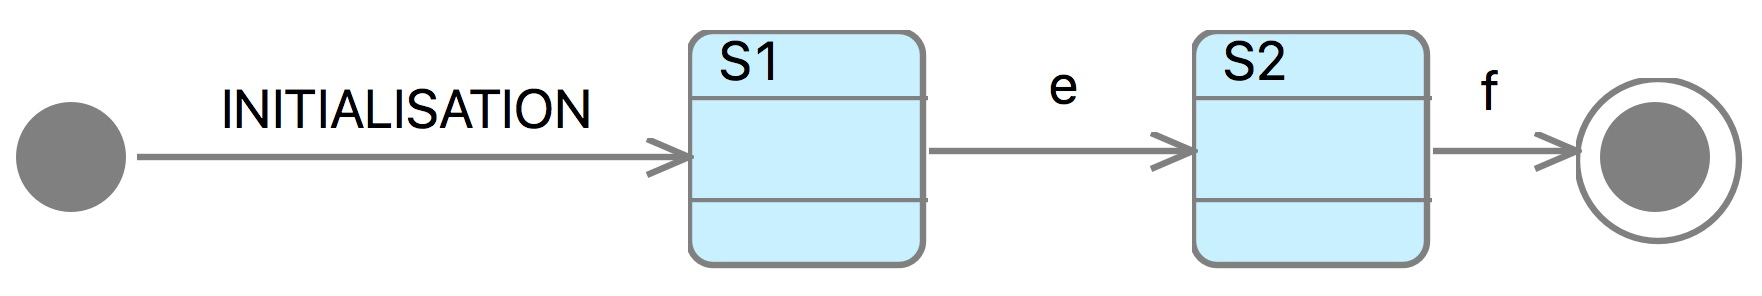
\includegraphics[width=0.6\textwidth]{figures/iumlb-SM}
	\caption{An example \iUMLB state-machine}
	\label{fig:iumlb-sm}
\end{figure}

Each state is encoded as a boolean variable and the current state is indicated by one of the boolean variables being set to |TRUE|. 
An invariant ensures that only one state is set to |TRUE| at a time.
%The state-machine, is initialised by setting one state variable to |TRUE| and all others to |FALSE|.
Events change the values of state variables to move the |TRUE| value according to the transitions in the state-machine.  
The \EventB translation%
%
\footnote{%
  Here, $\mathrm{partition(S, T1, T2, \ldots)}$ means the set $S$ is partitioned into disjoint (sub-)sets $T1, T2, \ldots$.
that cover $S$} %
of the state-machine in Figure~\ref{fig:iumlb-sm} can be seen in Listing~\ref{lst:eventb-sm}.%
\begin{lstlisting}[caption={Translation of the state-machine in Fig.~\ref{fig:iumlb-sm}},label={lst:eventb-sm}, language=Event-B, escapechar=|, frame=single, float=t]
 variables S1 S2
invariants 
	TRUE !: {S1, S2} => partition({TRUE}, {S1}/\{TRUE}, {S2}/\{TRUE})
events
    INITIALISATION: begin S1, S2 := TRUE, FALSE end
    e: when S1 = TRUE then S1, S2 ≔ FALSE, TRUE  end
    f: when S2 = TRUE then S2 := FALSE end
end
\end{lstlisting}	
	
%%% Local Variables:
%%% mode: latex
%%% TeX-master: "../SCXMLREF"
%%% End:

% !TEX root = ../SCXMLREF.tex


\subsection{Intrusion Detection System}
\label{sec:secbot}


The simple intrusion detection system is designed using an Application-Specific Integrated Circuit (ASIC) which connects to a buzzer and a sensor over a Serial Peripheral Interface (SPI) bus. The system is controlled via the ASIC on the SPI bus. At power-up, the ASIC sends commands over the SPI bus to initialize the sensor and the buzzer. After waiting for 50 milliseconds the ASIC enters its main routine, which makes the buzzer respond to the sensor. In the early design phase the statechart model of this system may be limited to the ASIC that captures the initialization of the peripherals and the 50 ms wait. In the interest of simplicity we elide all details of the main routine.

A statechart model of this system is shown in figure~\ref{fig:ASIC}. The ASIC starts by initializing the buzzer, this involves sending a message over the SPI bus. These messages constitute an implementation detail that we elide at this abstraction level. Once the message is sent (which will be indicated by some event saying that the SPI system is done), the ASIC moves on to initialize the sensor. After the ASIC moves into a waiting state for 50 ms, and finally moves into the state which represents normal operation. At this abstraction the \textbf{spi\_done} triggered, which signals completion by the SPI system, is an internal trigger that can be fired at any time.

\begin{figure*}[t!]
    % \begin{centering}
	    \begin{subfigure}[t]{0.5\textwidth}
	        \begin{centering}
	        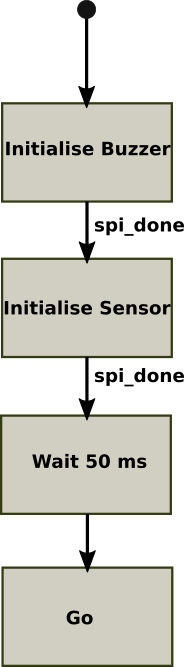
\includegraphics[height=3in]{figures/ASIC}
	        \caption{ASIC component high level abstraction}
	        \label{fig:ASIC}
	        \end{centering}
	    \end{subfigure}
\qquad
	    \begin{subfigure}[t]{0.5\textwidth}
	        % \begin{centering}
	        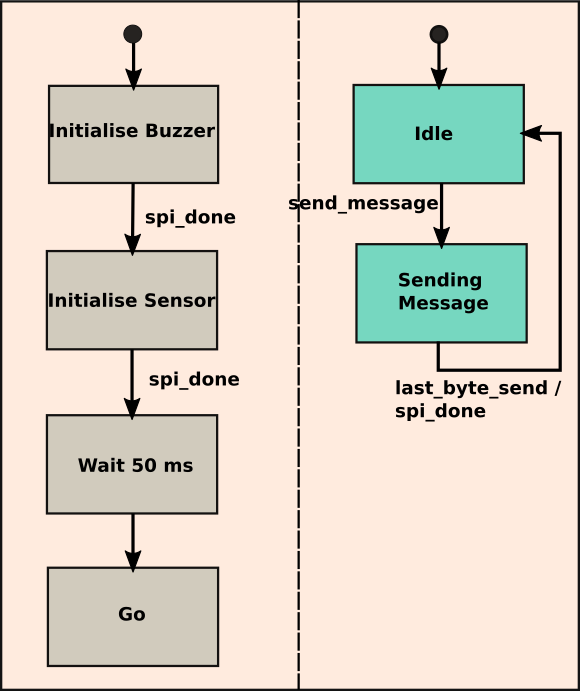
\includegraphics[height=3in]{figures/ASIC&SPI_1}
	        \caption{First refinement introducing the abstract model of the SPI subsystem.}
	        \label{fig:ASIC_SPI_1}
	        % \end{centering}
	    \end{subfigure}
	    \caption{Statechart diagram for Intrusion Detection System (SecBot) including the abstract representation of the ASIC and SPI components.}
    % \end{centering}
\end{figure*}

In a subsequent level of refinement, shown in figure~\ref{fig:ASIC_SPI_1}, the designer adds a parallel state representing the SPI subsystem. The SPI subsystem is usually on an \textbf{Idle} state until the \textbf{send\_message} trigger is raised, at which point the SPI subsystem enters a state \textbf{Sending Message}, which represents sending the message, byte by byte. When the last byte of the message is sent, it raises the \textbf{spi\_done} trigger, allowing the other parallel state to continue, while SPI subsystem returns to idle. In the current refined model the we have incorporated the implementation details for raising \textbf{spi\_done} and introduced a new internal trigger 
\textbf{send\_message}, which is nondeterministic at this point.

The model can be farther refined by incorporating more details on how the initialization states, the wait state, and the SPI subsystem operate, including how they interact with each other. The statechert diagram for this refinement level is in figure~\ref{fig:ASIC_SPI_2}. The \textbf{Initialize Buzzer} state constructs the SPI message to send, then raises the \textbf{send\_message} trigger, and then waits.
After \textbf{send\_message} is raised, the SPI subsystem reacts. It spins for a while in the \textbf{Send Byte} state, looping as many times as it takes to get to the last byte in the message. When the last byte in the message is sent, it goes back to \textbf{Idle} and raises an event which allows the state machine on the left to proceed. The sensor is then initialized in a very similar manner to the buzzer. After both peripherals are initialized, the state machine goes into the \textbf{Wait 50 ms} state, where it increments a counter until it reaches some maximum, then exits.

\begin{figure}[]
  \begin{centering}
  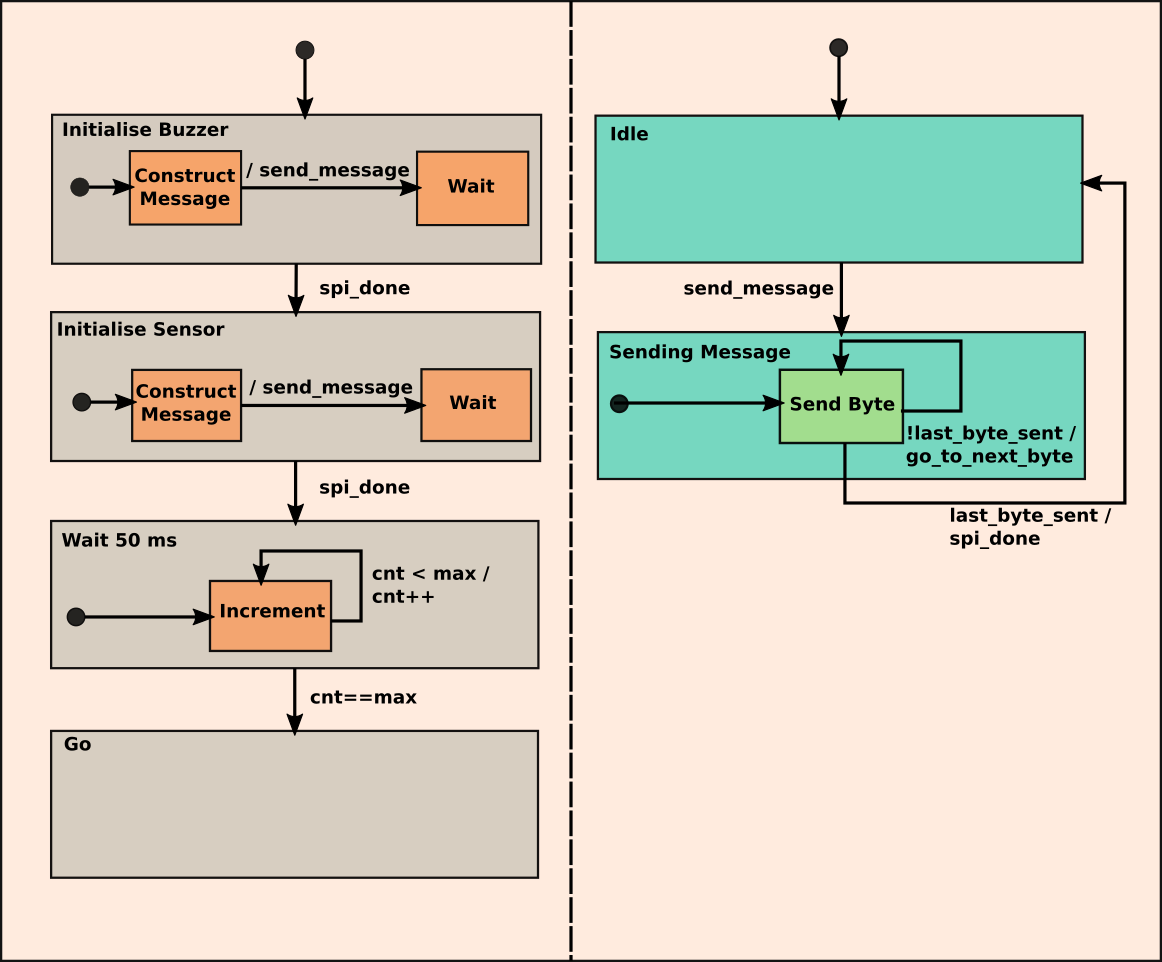
\includegraphics[width=0.8\textwidth]{figures/ASIC&SPI_2}
  \caption{Statechart diagram for Intrusion Detection System (SecBot) including implementation details for the messages send between the systems components.}
  \label{fig:ASIC_SPI_2}
  \end{centering}
\end{figure} 

The system described must send messages to complete the initialization of the buzzer and sensor, but once the main routine is reached (\textbf{Go} state) no more messages should be sent through the SPI bus. As a result, when the ASIC is in the \textbf{Go} state the SPI subsystem must be in the \textbf{Idle} state. This system property must be satisfied by the system model first refinement and any subsequent refinement representations of the system.

% Listing for XML
% \usepackage{listings}
% \usepackage{color}
 
\definecolor{dkgreen}{rgb}{0,0.6,0}
\definecolor{gray}{rgb}{0.5,0.5,0.5}
\definecolor{mauve}{rgb}{0.58,0,0.82}
\definecolor{gray}{rgb}{0.4,0.4,0.4}
\definecolor{darkblue}{rgb}{0.0,0.0,0.6}
\definecolor{lightblue}{rgb}{0.0,0.0,0.9}
\definecolor{cyan}{rgb}{0.0,0.6,0.6}
\definecolor{darkred}{rgb}{0.6,0.0,0.0}


\lstset{
  basicstyle=\ttfamily\footnotesize,
  columns=fullflexible,
  showstringspaces=false,
  numbers=left,                   % where to put the line-numbers
  numberstyle=\tiny\color{gray},  % the style that is used for the line-numbers
  stepnumber=1,
  numbersep=5pt,                  % how far the line-numbers are from the code
  backgroundcolor=\color{white},      % choose the background color. You must add \usepackage{color}
  showspaces=false,               % show spaces adding particular underscores
  showstringspaces=false,         % underline spaces within strings
  showtabs=false,                 % show tabs within strings adding particular underscores
  frame=none,                   % adds a frame around the code
  rulecolor=\color{black},        % if not set, the frame-color may be changed on line-breaks within not-black text (e.g. commens (green here))
  tabsize=2,                      % sets default tabsize to 2 spaces
  captionpos=b,                   % sets the caption-position to bottom
  breaklines=true,                % sets automatic line breaking
  breakatwhitespace=false,        % sets if automatic breaks should only happen at whitespace
  title=\lstname,                   % show the filename of files included with \lstinputlisting;
                                  % also try caption instead of title  
  commentstyle=\color{gray}\upshape
}


\lstdefinelanguage{XML}
{
  morestring=[s][\color{mauve}]{"}{"},
  morestring=[s][\color{black}]{>}{<},
  morecomment=[s]{<?}{?>},
  morecomment=[s][\color{dkgreen}]{<!--}{-->},
  stringstyle=\color{black},
  identifierstyle=\color{lightblue},
  keywordstyle=\color{red},
  morekeywords={xmlns,xsi,noNamespaceSchemaLocation,type,id,x,y,source,target,version,tool,transRef,roleRef,objective,eventually}% list your attributes here
}
% Listing for XML

\begin{lstlisting}[caption=Snippet for SCXML representation of SecBot model,label={lst:secBot}, language=xml]
...
<state id="SecBot" iumlb:refinement="0">
    <parallel id="SecBot_parallel">

     	<!-- For ASIC component -->
    	<state id="ASIC" iumlb:refinement="0">
        	<initial iumlb:refinement="0">
          		<transition target="InitialiseBuzzer"/>
        	</initial>
        	<state id="InitialiseBuzzer" iumlb:refinement="2">
        		<initial iumlb:refinement="2">
	            	<transition target="IBConstructMessage"/>
	          	</initial>
          		<transition cond="" event="spi_done" target="InitialiseSensor"/>
          		<state id="IBConstructMessage" iumlb:refinement="2">
	            	<transition target="IBWait">
	              		<raise event="send_message"/>
	            	</transition>
          		</state>
          		<state id="IBWait" iumlb:refinement="2"/>
        	</state>
       		<state id="InitialiseSensor" iumlb:refinement="2">
        		...
        	</state>
        	<state id="Wait50ms" iumlb:refinement="2">
          		...
        	</state>
        	<state id="Go">
          		<iumlb:invariant name="spi_idle_in_Go" iumlb:predicate="Idle = TRUE" iumlb:refinement="1"/>
        	</state>
      	</state>

      	<!-- For SPI subsystem -->
      	<state id="SPI" iumlb:refinement="1">
	        <initial>
	        	<transition target="Idle"/>
	        </initial>
	        <state id="Idle">
				<transition event="send_message" target="SendingMessage">
					<iumlb:guard name="dontRaiseSpiDone" iumlb:predicate="spi_done ∉ SCXML_raisedTriggers" iumlb:refinement="1"/>
				</transition>
        	</state>
			<state id="SendingMessage">
				<transition cond="" event="last_byte_sent" target="Idle">
					<raise event="spi_done"/>
					<iumlb:guard name="dontRaiseSendMessage" iumlb:predicate="send_message ∉ SCXML_raisedTriggers" iumlb:refinement="1"/>
				</transition>
			</state>
		</state>
	</parallel>
</state>
...
\end{lstlisting}






% !TEX root = ../SCXMLREF.tex


\section{Intrusion Detection System}
\label{sec:secbot}

An \IDS is used to illustrate the use of refinement in \statecharts and how it is supported by \EventB verification tools.
The \IDS is designed using an \ASIC which connects to a buzzer and a sensor over a \SPI bus. The system is controlled via the \ASIC on the \SPI bus. At power-up, the \ASIC sends commands over the \SPI bus to initialise the sensor and the buzzer. After waiting for 50 milliseconds the \ASIC enters its main routine, which makes the buzzer respond to the sensor. In the early design phase the \statechart model of this system may be limited to the \ASIC that captures the initialisation of the peripherals and the 50 ms wait. In the interest of simplicity, we elide all details of the main routine.

A \statechart model of this system is shown in Fig.~\ref{fig:ASIC}. The \ASIC starts by initialising the buzzer, this involves sending a message over the \SPI bus. These messages constitute an implementation detail that we elide at this abstraction level. Once the message is sent (which will be indicated by some event saying that the \SPI system is done), the \ASIC moves on to initialise the sensor. After that the \ASIC moves into a waiting state for 50 ms, and finally moves into the state which represents normal operation. At this abstraction the \textbf{spi\_done} triggered, which signals completion by the \SPI system, is an internal trigger that can be fired at any time.

In a subsequent level of refinement, shown in Fig.~\ref{fig:ASIC_SPI_1}, the designer adds a parallel state representing the \SPI subsystem. The \SPI subsystem is usually on an \textbf{Idle} state until the \textbf{send\_message} trigger is raised, at which point the \SPI subsystem enters a state \textbf{Sending Message}, which represents sending the message, byte by byte. When the last byte of the message is sent, it raises the \textbf{spi\_done} trigger, allowing the other parallel state to continue, while \SPI subsystem returns to idle. In the current refined model we have incorporated the implementation details for raising \textbf{spi\_done} and introduced a new internal trigger 
\textbf{send\_message}, which is nondeterministic at this point.

\begin{figure*}[!tb]\centering
	    \begin{subfigure}[t]{0.3\textwidth}
	        \begin{centering}
	        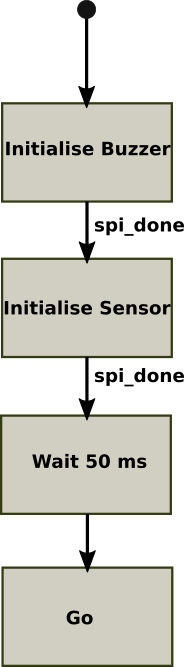
\includegraphics[height=2.5in]{figures/ASIC}
	        \caption{\ASIC component high level abstraction}
	        \label{fig:ASIC}
	        \end{centering}
	    \end{subfigure}
\qquad
	    \begin{subfigure}[t]{0.5\textwidth}
	        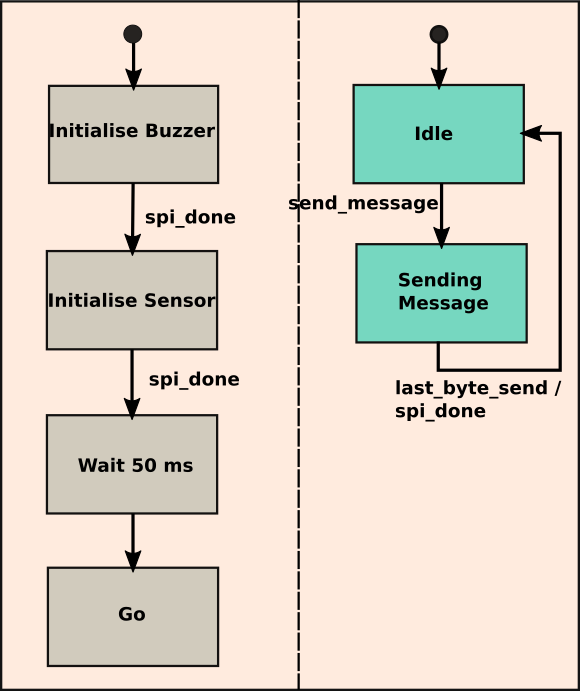
\includegraphics[height=2.5in]{figures/ASIC&SPI_1}
	        \caption{First refinement introducing the abstract model of the \SPI subsystem.}
	        \label{fig:ASIC_SPI_1}
	    \end{subfigure}
	    \caption{\Statechart diagram for \IDS including the abstract representation of the \ASIC and \SPI components.}
\end{figure*}

The model can be further refined by incorporating more details on how the initialisation states, the wait state, and the \SPI subsystem operate, including how they interact with each other. The \statechart diagram for this refinement level is in Fig.~\ref{fig:ASIC_SPI_2}. The \textbf{Initialise Buzzer} state constructs the \SPI message to send, then raises the \textbf{send\_message} trigger, and then waits.
After \textbf{send\_message} is raised, the \SPI subsystem reacts. It spins for a while in the \textbf{Send Byte} state, looping as many times as it takes to get to the last byte in the message. When the last byte in the message is sent, it goes back to \textbf{Idle} and raises an event which allows the state machine on the left to proceed. The sensor is then initialised in a very similar manner to the buzzer. After both peripherals are initialised, the state machine goes into the \textbf{Wait 50 ms} state, where it increments a counter until it reaches some maximum, then exits.

\begin{figure}[!tbp]
  \begin{centering}
  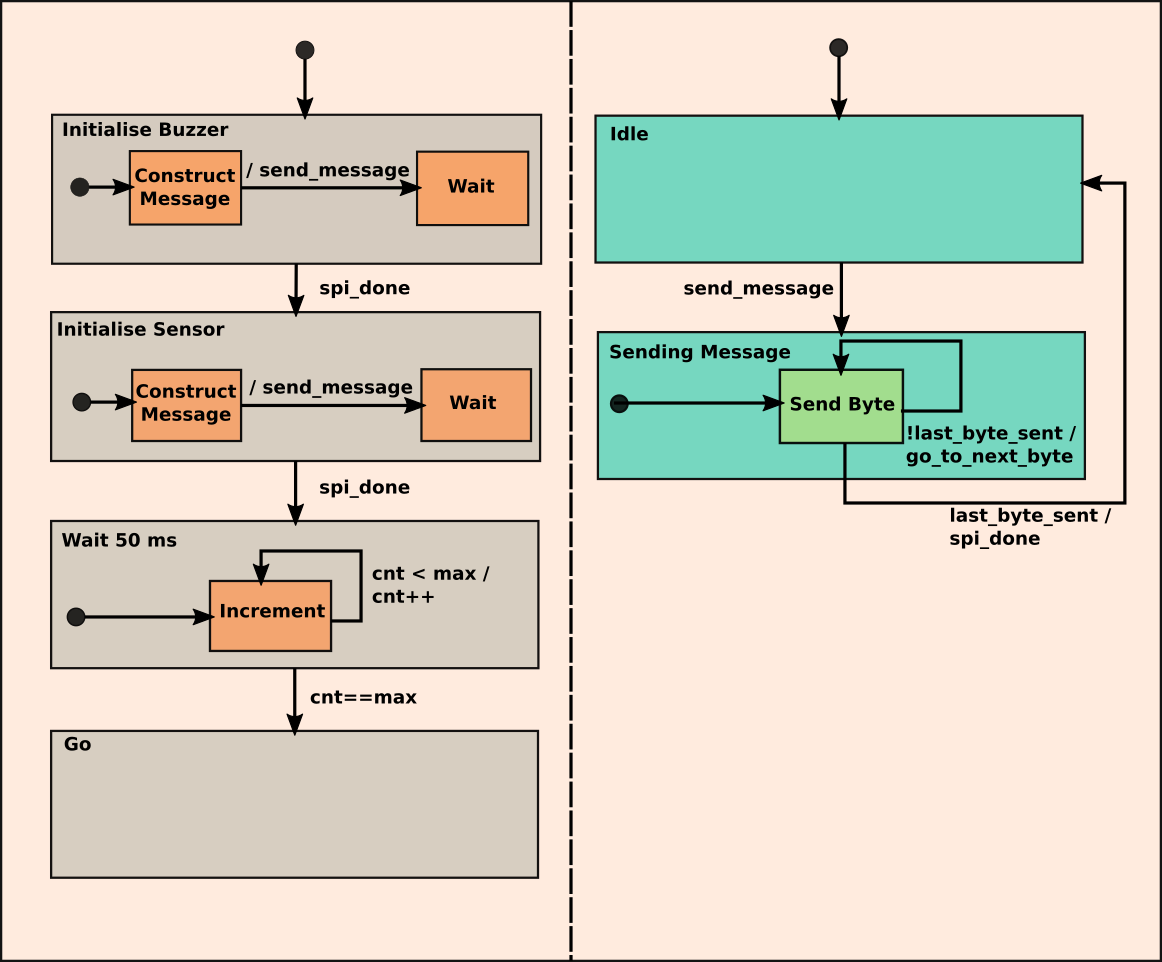
\includegraphics[width=0.8\textwidth]{figures/ASIC&SPI_2}
  \caption{\Statechart diagram for \IDS including implementation details for the messages send between the system components.}
  \label{fig:ASIC_SPI_2}
  \end{centering}
\end{figure} 

The system described must send messages to complete the initialisation of the buzzer and sensor, but once the main routine is reached (\textbf{Go} state) no more messages should be sent through the \SPI bus. As a result, when the \ASIC is in the \textbf{Go} state the \SPI subsystem must be in the \textbf{Idle} state. This system property must be satisfied by the system model first refinement and any subsequent refinement representations of the system.



%%% Local Variables:
%%% mode: latex
%%% TeX-master: "../SCXMLREF"
%%% End:



% !TEX root = ../SCXMLREF.tex

\section{Discussion}
\label{sec:discussion}

%This is the discussion...
%Compare the behaviour of a visually similar statechart (SecBot?) in \iUMLB and \SCXML 
%	Based on their \EventB translations
%	Using the theorem prover to test whether they are equivalent (they are not)
%	Using the model checker to compare traces
%	Using LTL to show that certain temporal properties are not achieved by the \iUMLB version.
%
%
%Early attempts – 
%1)	Simple next step – based on negated guards – negation is weakened
%2)	Engine – improves the R2C semantics but still suffers from the negated guards problem (refinement of the user model kinda works – simulations at the user level).
%\ColinCommented{IF POSSIBLE? use the secbot example to illustrate the problem of guard stengthening on refinement}
%
%The solution:
%3)	Transition combinations approach – works because there is always one event to completion. Invariants as well as simulations. 
%a.	Explosion – mitigated by mutual exclusions… same trigger – different state-chart regions.
%
%What can we do with it? 
%	Why is RTC needed?
%	Refinement in RTC


In order to introduce a notion of refinement into \SCXML we need to consider the kinds of things we would like to do in refinements and what properties should be preserved.
In practice we wish to leverage existing \EventB verification tools and hence adopt a notion of refinement that can be automatically translated into an equivalent \EventB model consisting of a chain of refinements. While it might be possible to utilise data refinement by replacing a state-chart with an alternative one, this would greatly complicate things and is impractical when the \SCXML model is a single state-chart (rather than a chain of refined models). Hence we start from the following requirements which allow superposition refinements and guard strengthening in \SCXML models:
\begin{itemize}
	\item The firing conditions of a transition can be strengthened by adding further textual constraints about the state of other variables and statemachines in the system.
	\item The firing conditions of a transition can be strengthened by being more specific about the (nested) source state,
	\item Nested state-charts can be added in refinements.
	\item Ancilliary data can be added and corresponding actions to alter it added to transitions.
	\item Raise actions can be added to transitions to define how internal triggers are raised. These internal triggers may have already been introduced and used to trigger transitions in which case they are non-deterministically raised at the abstract levels. (Note that external triggers are always unguarded and cannot be refined).
	\item Invariants can be added to states to specify properties that hold while in that state.
\end{itemize}

Refinement should preserve the value of the abstract state after each micro-step and at the end of each macro-step. The abstract state should not be altered by any new micro-steps that are introduced into an abstract macro-step, nor by any new macro-steps that are introduced. (Note that these goals take the view that macro-steps should align through refinement. An alternative approach that we are considering for future work takes the view that the macro-steps need not align and a micro-step may shift from one macro-step to another in a refinement). 

There seems to be an inherent difficulty with refining `run to completion' semantics which require that every enabled micro step, is completed before the next macro step is started. The problem is that, in a refinement, we want to strengthen the conditions for a micro step. However, by making the micro steps more constrained we disable them and make their completion more easily achieved. This makes the guard for taking the next macro step weaker breaking the notion of refinement.








\ColinCommented{Here we should discuss the various translations that we have tried illustrating the problems of getting a refinment. Mainly the idea of having a scheduling engine that moves the transition guards to a scheduler and fires a collection of enabled transitions before moving to the next step, versus the flattened
combinations approach that we finally adopted.}




% !TEX root = ../SCXMLREF.tex

\section{Extensions to \SCXML}
\label{sec:extensions}
 
The following syntax extensions are added to \SCXML models to support modelling features needed in \iUMLB/\EventB. These extensions are prefixed with `iumlb:' in order to distinguish them from the \SCXML XML parser. (So that they are ignored by \SCXML simulation tools). 
%They are loaded by EMF as generic feature maps (‘Any’ for contained elements and ‘AnyAttribute’ for attributes).
\begin{itemize}
	\item \textbf{iumlb:refinement} - an integer attribute representing the refinement level at which the parent element should be introduced (see Listing~\ref{lst:secBot}, line~\ref{line:refinement}).
	\item \textbf{iumlb:invariant} - an element that generates an invariant in \iUMLB. This provides a way to add invariants to states so that important properties concerning the synchronisation of state with ancilliary data and other state machines can be expressed (see Listing~\ref{lst:secBot}, line~\ref{line:invariant}).
	\item \textbf{iumlb:guard} - an element that generates a transition guard in \iUMLB. 
	This provides a way to add new guard conditions to transitions over several refinement (Listing~\ref{lst:secBot}, line~\ref{line:guard}) as well as providing an element with attributes such as derived (for \EventB theroems), name and comment.
	\item \textbf{iumlb:predicate} - a string attribute used for the predicate of a guard or invariant (Listing~\ref{lst:secBot}, line~\ref{line:predicate}).
\end{itemize}
Other attributes useful for \iUMLB elements: name, derived, type, comment, have also been added for convenience.

\begin{lstlisting}[caption={\textbf{Wait50ms} state snippet of \SCXML model representation illustrating the use of different \SCXML modeling features, as well as, added syntax extensions},label={lst:secBot}, language=xml, escapechar=|, frame=single]
...
<state id="Wait50ms" iumlb:refinement="2">
	<initial iumlb:refinement="2"> |\label{line:refinement}|
		<transition cond="cnt=0" target="Increment"/> 
	</initial>
	<iumlb:invariant name="check_cnt" iumlb:predicate="cnt &lt; max" iumlb:refinement="2"/> |\label{line:invariant}|
	<transition cond="" target="Go" iumlb:refinement="0" />
	<state id="Increment" iumlb:refinement="2">
		<transition cond="" event="tick" target="Increment">
			<assign attr="cnt" expr="cnt+1" location="cnt"/>
			<iumlb:guard name="stillCounting" iumlb:predicate="cnt &lt; 5"/> |\label{line:predicate}|
		</transition>
		<transition cond="" target="WAITDone">
			<iumlb:guard name="doneCounting" iumlb:predicate="cnt = 5"/> |\label{line:guard}|
    	</transition>
	</state>
	<final id="WAITDone" iumlb:refinement="2"/>
	<datamodel>
		<data expr="0" id="cnt" src="" iumlb:type="NAT "/>
	</datamodel>
</state>
...
\end{lstlisting}

Hierarchical nested state charts are translated into similarly structured \iUMLB state-machines. The generated \iUMLB model contains refinements that add nested state-machines as indicated in the  \SCXML \statechart (see Listing~\ref{lst:secBot}) by the \textbf{iumlb:refinement} attributes annotated on state elements. \iUMLB transitions are generated for each \SCXML transition and linked to \EventB events that represent each of the possible synchronisations that could involve that transition.


%%% Local Variables:
%%% mode: latex
%%% TeX-master: "../SCXMLREF"
%%% End:

% !TEX root = ../SCXMLREF.tex

\section{\SCXML Translation}
\label{sec:translation}

A tool to automatically translate \SCXML models into \iUMLB has been produced. 
The tool is based on the \EMF and uses an \SCXML metamodel provided by Sirius~\cite{siriuswebsite} which has good support for extensibility. 
The tooling for \iUMLB and \EventB already contains \EMF metamodels and provides a generic translator framework which has been specialised for the \SCXML to \iUMLB translation. 

Each \SCXML transition is translated into a corresponding \iUMLB transition. 
Fig.~\ref{fig:iumlb-verif} shows the \iUMLB representation, first refinement level design, of the \IDS described in
Fig.~\ref{fig:ASIC_SPI_1}. 
In the translation from \iUMLB to \EventB the `run to completion' semantics is supported by \EventB through the construction of a basis that constitutes an abstract execution model, which all designed systems refine. 
The basis includes \EventB \emph{context} and \emph{machine}. 
The context, shown in~\ref{lst:BasisContext}, defines the basis triggers as a partition of internal and external triggers, declared as |SCXML_FutureInternalTrigger| and |SCXML_FutureExternalTrigger| respectively. 
The abstract model of the \IDS extends the basis context and declares a new axiom that defines the partitions of the |SCXML_FutureInternalTrigger| set, which would include the \textbf{spi\_done} trigger and a new partition |SCXML_FutureInternalTrigger0| to enable the introduction of additional internal triggers by subsequent refinements as shown in line~\ref{line:refPartition} of Listing~\ref{lst:SecBotCont0}. 

\begin{lstlisting}[caption={Abstract basis context},label={lst:BasisContext}, language=Event-B, escapechar=|, frame=single]
context
	basis_c 	// (generated for SCXML)
sets
	SCXML_TRIGGER	 // all possible triggers
constants
	SCXML_FutureInternalTrigger	 // all possible internal triggers
	SCXML_FutureExternalTrigger	 // all possible external triggers  
axioms
	partition(SCXML_TRIGGER, SCXML_FutureInternalTrigger, SCXML_FutureExternalTrigger) 
end
\end{lstlisting}	

\begin{lstlisting}[caption={Context for \IDS abstract model},label={lst:SecBotCont0}, language=Event-B, escapechar=|, frame=single]
context
	IDS_Model_0_ctx //(generated from:/IDS_generated/secbot.scxml)
extends
	basis_c 
constants
	SCXML_FutureInternalTrigger0	
	SCXML_FutureExternalTrigger0
	spi_done	 	//trigger
axioms
	SCXML_FutureExternalTrigger0=SCXML_FutureExternalTrigger
	partition(SCXML_FutureInternalTrigger, SCXML_FutureInternalTrigger0,{spi_done}) |\label{line:refPartition}|
end
\end{lstlisting}

The basis machine, partially shown in Listing~\ref{lst:BasisMachine}, declares the variables that correspond to the triggers present in the queue at any given time, as well as, the |SCXML_uc| flag, which signals when a run to completion macro-step has been completed and no un-triggered transitions are enabled. 
At the point of initialization, both queues are empty and |SCXML_uc| is set to false. 
The parametric |SCXML_futureExternalTrigger| event updates the external trigger queue with any newly raised trigger. 
To raise an external trigger, each external trigger in the model must extend this event.   
The |SCXML_futureInternalTransitionSet| basis event must be refined by any event in the model conditioned on an internal trigger. 
The guards of this event check for the completion of the previous macro-step. 
A similar behavior is followed by |SCXML_futureExternalTransitionSet| event, if no internal triggers are in the queue.  

\begin{lstfloat}
\begin{lstlisting}[caption={Snippet of abstract basis machine}, label={lst:BasisMachine},language=Event-B, escapechar=|, frame=single][t]
machine 
	basis_m   // (generated for SCXML)
sees 
	basis_c 
variables
	SCXML_iq	  // internal trigger queue
	SCXML_eq	  // external trigger queue
	SCXML_uc	  // run to completion flag
invariants
	SCXML_iq ⊆ SCXML_FutureInternalTrigger	// internal trigger queue
	SCXML_eq ⊆ SCXML_FutureExternalTrigger	// external trigger queue
	SCXML_iq ∩ SCXML_eq= ∅					// queues are disjoint
	SCXML_uc ∈ BOOL							// completion flag
events

	INITIALISATION: 
	begin
		SCXML_iq := {}		//internal Q is initially empty
		SCXML_eq := {}		//external Q is initially empty
		SCXML_uc := FALSE	//completion is initially FALSE
	end

	SCXML_futureExternalTrigger: 
	any SCXML_raisedTriggers where
		SCXML_raisedTriggers ⊆ SCXML_FutureExternalTrigger 
	then
		SCXML_eq ≔ SCXML_eq ∪ SCXML_raisedTriggers 
	end
	
	SCXML_futureInternalTransitionSet: 
	any SCXML_it SCXML_raisedTriggers where
		SCXML_it ∈ SCXML_iq 
		SCXML_uc = TRUE 
		SCXML_raisedTriggers ⊆ SCXML_FutureInternalTrigger 
	then
		SCXML_uc ≔ FALSE 
		SCXML_iq ≔ (SCXML_iq ∪ SCXML_raisedTriggers) ∖ {SCXML_it} 
	end

	SCXML_futureUntriggeredTransitionSet: 
	any SCXML_raisedTriggers where
		SCXML_uc = FALSE
		SCXML_raisedTriggers ⊆ SCXML_FutureInternalTrigger
	then
		SCXML_uc ≔ FALSE 
		SCXML_iq ≔ SCXML_iq ∪ SCXML_raisedTriggers 
	ends

end
\end{lstlisting}
\end{lstfloat}
To completely control the execution flow of the model, all un-triggered transitions must refine the |SCXML_futureUntriggeredTransitionSet| event. 
Any of the previously discussed events can raise a set of internal triggers, |{i1,i2...}|, by introducing a guard that defines |{i1,i2...} <: SCXML_raisedTrigger| parameter (not shown in listings). 
As shown in listing~\ref{lst:SecBotMach0} an event that corresponds to a triggered transition uses the provided parameter |SCXML_it| (|SCXML_et| for externally triggered transitions) to define which trigger enables the event (see line~\ref{line:defTrigger}).

\begin{lstlisting}[caption={Event-B event corresponding to internal triggered transition to \textbf{Wait50ms} state in refinement level 1 shown in Fig.~\ref{fig:ASIC}}, label={lst:SecBotMach0},language=Event-B, escapechar=|, frame=single]
spi_done__InitialiseSensor_Wait50ms:	
refines SCXML_futureInternalTransitionSet 
any SCXML_it SCXML_raisedTriggers where
	SCXML_it  ∈ SCXML_iq 
	SCXML_uc = TRUE
	SCXML_raisedTriggers ⊆ SCXML_FutureInternalTrigger
	InitialiseSensor = TRUE
	SCXML_it = spi_done  	//trigger for this transition |\label{line:defTrigger}|
then
	SCXML_uc ≔ FALSE
	SCXML_iq ≔ (SCXML_iq ∪ SCXML_raisedTriggers) ∖ {SCXML_it}
	InitialiseSensor ≔ FALSE
	Wait50ms ≔ TRUE
end
\end{lstlisting}

%%% Local Variables:
%%% mode: latex
%%% TeX-master: "../SCXMLREF"
%%% End:

% !TEX root = ../SCXMLREF.tex

\section{Application to Intrusion Detection System}
\label{sec:example}
The SecBot example : pics from slides

Note why it would not be a refinement 

A tool to automatically translate \SCXML models into \iUMLB has been produced. The tool is based on the Eclipse Modelling Framework (EMF) and uses a an \SCXML metamodel provided by Sirius~\cite{siriuswebsite} which has good support for extensibility. The tooling for \iUMLB and \EventB already contains EMF metamodels and provides a generic translator framework which has been specialised for the \SCXML to \iUMLB translation.  

Proving properties in SCXML

Properties about the synchronisation of parallel state-machines (such as ASIC=Go => SPI=IDLE and ASIC=Wait50ms => SPI=IDLE) can be difficult to verify for all scenarios via simulation in SCXML. Proof of such properties is a major benefit of translating into Event-B.  Furthermore in order to benefit from the abstraction provided by Event-B, we would like to prove such things at abstract levels before the complication of further details are introduced. 
2.	To prove POs about not raising specific internal triggers in abstract 'future' events – the translation can 'look ahead' at the future refinements and add a guard excluding specific internal triggers from being raised in a state if they are not raised in any contained substates/transitions. Alternatively, they could be automatically generated and added to satisfy all user invariants concerning the raising of internal triggers regardless of whether they are violated in future levels. If it is not obeyed by future transtions, guard strengthening GD proof obligations will make it obvious where the problems lie. For example, the guard… 
     $Go = TRUE \limp send\_message \notin SCXML\_iq’$	
     (where SCXML\_iq’ is the new value to be assigned to SCXML\_iq in the event’s actions)
needs to be automatically added to all the future transitionSet events to prove they do not break the property in 1. This could be automatically generated and added to satisfy all user invariants concerning the raising of internal triggers. If it is not obeyed by future transtions, guard strengthening GD proof obligations will make it obvious where the problems lie.
3.	Add a way to exclude specific internal triggers from ever being raised by a user transition (e.g. a doesn't raise element) - Or can this be automatically generated like 1). For example, the guard… 
     send\_message ∉ SCXML\_raisedTriggers
needs to be added to the transition Wait50ms\_Go in order to prove that it does not violate the property ASIC=Go => SPI=IDLE. However, if this is to be done manually, we would need a notation that avoids the user having to know about the internal basis parameter, SCXML\_raisedTriggers.
4.	There are still things to consider about proving these properties are true at an abstract level - that is, you cannot prove them unless you add the detail that makes them true!! (example :- detail about when we raise send\_message is in level 2 but we need it to prove no messages get in the queue after SPI raises the second spi\_done). However, invariants and guards can be added at the abstract level in order to abstractly add the necessary constraints to make a proof. If these constraints are not maintained in later levels, simpler proof obligations about guard strengthening will be unprovable. These abstract guards should be removed at later refinements when the details have been specified. This implies using ranges in refinement attributes which we have considered but not used in the past.



% !TEX root = ../SCXMLREF.tex

\section{Conclusion}
\label{sec:conclusion}
We have shown how a slightly extended and annotated \statechart, with a typical 'run to completion' semantic, can be translated into the \EventB notation for verification of synchronisation properties using the \EventB theorem proving tools.
Furthermore, borrowing from the refinement concepts of \EventB, we introduce a notion of refinement to \statecharts and demonstrate how the proof of a property at an abstract level, helps formulate constraints that must apply (and will be verified to do so) in further refinements.

\SonAdd{%
  Refinement of UML \mbox{\statecharts} has been  studied previously in~\mbox{\cite{DBLP:journals/corr/HansenSL15,1347517,szasz10:_behav_refin_uml_statec}}. 
  In~\mbox{\cite{DBLP:journals/corr/HansenSL15}}, the authors propose  a ``purely additive'' refinement process where no elements (e.g. events, guards, etc.) of the original model can be removed and the ``external'' behaviour of the model is therefore preserved.  
  This refinement process is similar to \mbox{\EventB} ``superposition'' refinement which we use in our translation.  
  In~\mbox{\cite{1347517}}, the authors consider a coalgebraic description of UML \mbox{\statecharts}, and define an equivalence relationship and a behavioural refinement notion between \mbox{\statecharts}.  In~\mbox{\cite{szasz10:_behav_refin_uml_statec}}, the authors define a structured operational semantics of \mbox{\statecharts} based on label transition systems.  
  Behaviour refinements are then constructed based on this semantics. 
  The authors prove that a ``safe-extension'' of UML \mbox{\statecharts} is a correct behavioural refinement.  
  In our paper, we focus on the run-to-completion semantics of \mbox{\statecharts}, whereas none of the above work deals with it explicitly. 
  Furthermore, the refinement process supported in~\mbox{\cite{DBLP:journals/corr/HansenSL15,1347517}} is based on refinement patterns (called refinement rules/laws), whereas we rely on the more general theory of refinement, given by the proof obligations of \mbox{\EventB}, for proving the refinement relationship between \mbox\statecharts.
}

In future work we will continue to experiment with different examples to explore the alternative translation strategies in more detail. 
In particular, further work on refinement of the micro/macro-step and whether correspondence of macro-steps can be relaxed; whether more complex refinement techniques could be supported (for example, using ranges in refinement annotations) would be useful; supporting/comparing alternative variations of semantics (by generating a different basis/scheduler for the translation).

For our interpretation of \statecharts in \mbox{\iUMLB}, we used the `run-to-completion' semantics of \statecharts.  In particular, we have carefully designed our translated model such that the semantics is captured as a generic abstract model, which is subsequently refined by the translation of the \SCXML model.  An advantage of this approach is that we can easily adapt the basis model with other alternative semantics~\mbox{\cite{Eshuis_2009}} without changing the translation of the \SCXML model. 

While \statecharts interpreted in \iUMLB provide a way to incorporate refinement in an intuitive way, reversing this to \emph{discover} refinements holds promise. 
Checking a particular \statechart model for hierarchical structures that happen to follow the refinement proof obligations suggests an automatic way to accomplish abstract interpretation on an existing model.  
Such discovered abstraction/refinement relationships might improve the scalability of more complex \statechart models ``for free''.
%%% Local Variables: 
%%% mode: latex
%%% TeX-master: "../SCXMLREF.tex"
%%% End: 


%\begin{footnotesize}
\begin{scriptsize}
	\vspace{6 pt}
	\noindent
	All data supporting this study are openly available from the University of Southampton repository at
	https://tinyurl.com/SCXML-REF    \textbf{(DOI FOR FINAL)}
	%http://doi.org/10.????/SOTON/D0???\\   %<GET a new DOI!!>

\end{scriptsize}
\begin{footnotesize}
\vspace{6 pt}
\noindent
\textbf{Acknowledgment:} The authors would like to thank Jason Michnovicz for developing the \IDS example used throughout the manuscript.

\par

\end{footnotesize}
%\end{scriptsize}

\bibliographystyle{plain}
\bibliography{SCXMLREF}

\end{document}

%%% Local Variables: 
%%% mode: latex
%%% TeX-master: t
%%% End: 
